\chapter{Estado del Arte\label{sec:estado_del_arte}}


\textcolor{rositaoscuro}{asdf}
\textcolor{teal}{sdffsd}


En este capítulo se estudia más detalladamente el problema que pretende resolver el proyecto y las características del entorno.


%--Enfermedades
\section{Enfermedades neurológicas}
\label{sec:dolencias2}

Las enfermedades neurológicas son muy frecuentes en España. Los servicios de neurología atienden a más de 2.2 millones de pacientes al año. Además, 7.5 millones de personas sufren algún tipo de enfermedad neurológica (un 16\% de la población española). 

Se conocen dos tipos de accidentes cerebrovasculares (ACV) según la causa \cite{tipoIctus}:
\begin{itemize}
	\item Hemorragia cerebral: suceden  a causa de la rotura de una vaso sanguíneo.
	\item Isquemia cerebral: consecuencia de una obstrucción de una arteria por la presencia de un coágulo de sangre. En muchas ocasiones se origina en el corazón y se desplaza hasta el cerebro, dónde interrumpe el flujo sanguíneo.
\end{itemize}

Sea cual sea la causa del ictus, el daño cerebral adquirido puede ser irreversible. Las secuelas posteriores pueden repercutir considerablemente en la calidad de vida del afectado.

Cuando se sufre un accidente cerebrovascular es recomendable recibir atención neurológica temprana, preferentemente durante la primera hora. Cuanto más tiempo se tarde en recibir atención por un especialista, peores serán las consecuencias del accidente y más complicada la recuperación.

Este tipo de enfermedades habitualmente son atendidas por los servicios de urgencias, debido a que se surge de manera fortuita y son efectos instantáneos son de gran magnitud. De los 26 millones de urgencias hospitalarias que se atienden al año en España, el 14\% son neurológicas y en su gran mayoría son consideradas de nivel I-III (riesgo vital-riesgo potencial). Asimismo, neurología es la segunda especialidad más requerida en los servicios de urgencias.

Existe una medida denominada DALY (años de vida ajustados por discapacidad) que estima el número de años perdidos a una enfermedad, discapacidad o muerte prematura. Según la cual sitúa el ICTUS como la más influyente (con el 55\% entre las demás) de entre dolencias como: alzheimer (12\%), migraña (8.3\%), epilepsia (7.9\%), parkinson, esclerosis múltiple, meningitis y otros. Este hecho señala la importancia de conseguir poner remedio a esta situación, consiguiendo que el ictus no fuera tan significativo en este tipo de medidas.

El ictus tiende a prevalecer más en el enfermo cuanto mayor es su edad. Es decir, cuanto mayor edad tiene la persona afectada, más difícil es la recuperación de este.

\cite{pentienII}

\subsection{Secuelas}
\label{sec:secuelas}

Los afectados por esta enfermedad padecen tras sufrirla una serie de secuelas físicas y sensoriales de difernetes tipos que se citan a continuación:

\begin{itemize}[label=$ \rhd $]
	\item Alteraciones de tono muscular:
	\begin{itemize}[label=$ \longrightarrow $]
		\item Espasticidad
		\item HIpertonía
		\item Hipotomía
		\item Distonía
		\item Pérdida de simetría
		\item Movimiento enlentecido
		\item Movimiento en bloque
		\item Alteraciones en la cooredinación
		\item Luxaciones / subluxaciones
		\item Edema
	\end{itemize}
	\item Paresia o parálisis
	\begin{itemize}[label=$ \longrightarrow $]
		\item Monoplejia
		\item Hemiplegia / Hemiparesia
		\item Paraplegia
		\item Tetraplejia / Tetraparesia
	\end{itemize}
	\item Pérdida de las sensaciones táctiles y propioceptivas
	\item Fatiga
	\item Alteraciones de equilibrio y coordinación
\end{itemize}

Cuando una persona sufre una enfermedad neurológica son varios los aspectos de sus vida en los que necesita ayuda para volver a llevar una vida autonoma. Necesita cuidado médico para revisar el estado de su salud personal. Para mejorar la comunicación con el entrono el paciente necesita de logoterapia y terapia ocupacional. Además, existe una necesidad psicosocial que se resuelve mediante grupos de apoyo y soporte familiar.

Por último, la cuestión en la que se centra este trabajo: el control en la mejora de la condición física del paciente para conseguir autonomía en la vida diaria a través de rehabilitación a largo plazo. Actividad que es guiada gracias a los profesionales fisioterapeutas.

\subsection{Rehabilitación}
\label{sec:neuronal2}

Tras el alta hospitalaria el paciente requiere un largo periodo de rehabilitación para poder realizar tareas cotidianas como\cite{secuelasIctus}:
\begin{itemize}
	\item Subir escaleras
	\item Vestirse
	\item Ir al baño
	\item Asearse
	\item Alimentarse
	\item Pasear
\end{itemize}

Para poder lograr minimizar los impedimentos físicos que experimentan estos pacientes la rehabilitación juega un papel fundamental. Esto ayuda además a la recuperación de la vida social de estas personas. 

Existen muchos tipos de técnicas de tratamiento para fomentar el trabajo de las funcionalidades de las extremidades superiores. A continuación s eprocede a exponer brevemente algunas de ellas:

\begin{itemize}[label=$ \rhd $]
	\item \textbf{Técnicas manuales} Consisten en el uso de la actividad como medio y fin.
	\item \textbf{Entrenamiento motor orientado a tareas}
	\item \textbf{Ferulaje}
	\item \textbf{Vendaje neuromuscular}
	\item \textbf{Electroestimulación funcional} Se estimulan los músculos mediante impulsos electricos para que este se mueva.
	\item \textbf{Mirror therapy} Se pone un espejo entre las dos extremidades, reflejando la mano que tiene capacidad de movimiento. El ejercicio consiste en mover la mano sana para estimular mediante el espejo a que el cerebro muevo la otra.
	\item \textbf{Realidad virtual}
	\item \textbf{Rehabilitación robótica}
\end{itemize}


%--Enfermedades
\section{El papel de las manos}
\label{sec:manos2}

De entre las seis actividades de la vida diaria expuestas en el punto anterior, para poder realizar cuatro de ellas es necesario poder tener el control del movimiento de las manos. En sí, se utilizan las manos para muchísimas más tareas de la vida cotidiana, pero en este marco se procura primero recuperar la capacidad mínima para poder valerse por uno mismo en las tareas más básicas y vitales.



\subsection{Fundamentos de las manos}
\label{sec:fuindamentos2}

Las manos son una parte del cuerpo humano con una funcionalidad muy importante en el día a día de las personas. En la figura \ref{fig:anatomiaMano} se observan las falanges que componen las manos. 

\begin{figure}[H]
	\centering
	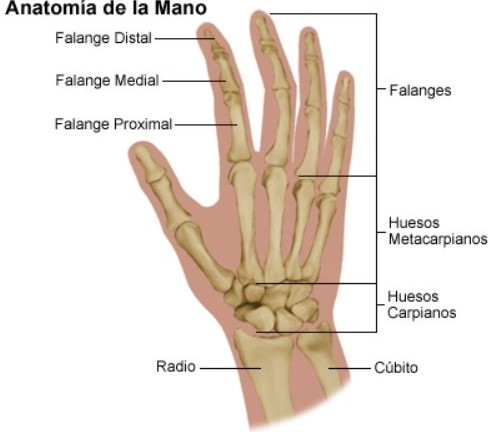
\includegraphics[width=0.5\textwidth]{./img/anatomiaMano}
	\caption{Anatomía de las manos.  \cite{imgAnatomiaMano}}
	\label{fig:anatomiaMano}
\end{figure} 

Cuando un persona ha sufrido un ictus en muchas ocasiones pierde la movilidad total o parcial de la mano. Es importante comprender que en este tipo de afecciones el problema no se inicia en un defecto físico de la mano, sino que son los músculos que a consecuencia del ACV han deshabilitado la capacidad de enviar pulsos eléctricos a esta extremidad. Estos son los pulsos eléctricos, entendidos como las señales que envía el cerebro a la mano para que esta se mueva. Lo que se pretende recuperar mediante rehabilitación es esta comunicación entre el cerebro y el músculo. Esto no significa que las manos no necesiten recuperar la capacidad física de movimiento, ya que cuanto más tiempo pasa un músculo sin moverse, este va perdiendo habilidad para moverse. Por ello, es muy importante trabajar el movimiento de los músculos aunque estos no sean capaces de moverse por si mismos.

%--REHABILITACIÓN
\subsection{Rehabilitación de las manos}
\label{sec:Rehabilitacion2}

Gracias a la rehabilitación del tren superior, aunque el paciente no recupere la capacidad de andar será capaz de resolver muchas situaciones cotidianas. El objetivo es recuperar la máxima funcionalidad de las extremidades superiores. Lo que resulta en mejorar el rango de movimiento activo y parámetros como fuerza, coordinación, sensibilidad y destreza manipulativa.

Dentro de la rehabilitación de las manos se pueden utilizar las técnicas nombradas anteriormente. Durante las rehabilitaciones hace falta realizar muchos tipos de movimientos. En la figura \ref{fig:movManos} se representan los movimientos de las manos. Estos movimientos debería de ser capaz de realizar un prototipo que tenga por función de medir el movimiento de las manos adherido a estas:

\begin{figure}[H]
	\centering
	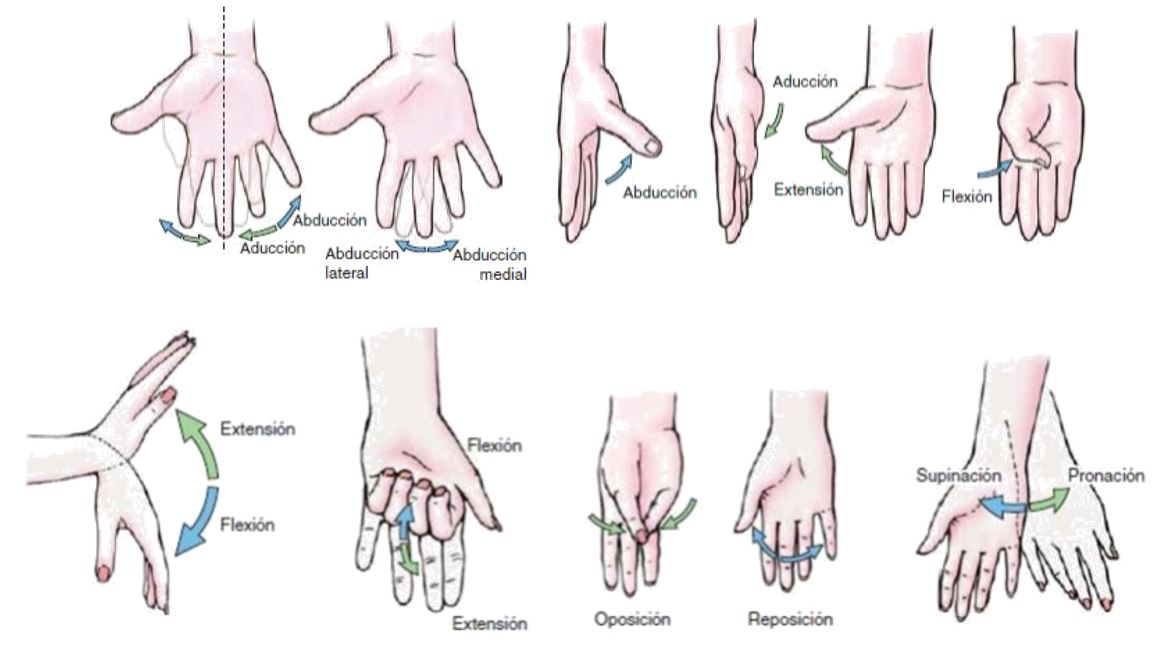
\includegraphics[width=0.85\textwidth]{./img/ejerciciosRehManp}
	\caption{Movimientos de las manos \cite{movimientoMano}} 
	\label{fig:movManos}
\end{figure}




\section{Captura del movimiento}
\label{sec:captura2}

Para mejorar el proceso de rehabilitación resulta imprescindible avaluar el avance de las sesiones. Actualmente se utilizan mecanismos de medida que no resultan precisos (ver figura \ref{fig:medidaAnticuada}). Los datos obtenidos de estas mediciones no son lo suficientemente fiables como para que pueda cuantificarse realmente el avance de la condición del paciente.

La solución a este cuestión es un sistema de medida capaz de realizar una valoración objetiva de la evolución de los pacientes. Lo cual permitiría al personal rehabilitador diseñar sesiones de rehabilitación más específicos para cada paciente y tener un mejor conocimiento d la repercusión de los ejercicios de rehabilitación en los pacientes. Mejorando además las prescripciones realizadas. 

Este tipo de dispositivo se debe conseguir mediante el empleo de nuevas tecnologías incipientes. Es un buen momento para innovar en este ámbito ya que en estos últimos años se ha detectado un incremento de desarrollo tecnológico en el ámbito médico debido a las mejoras del servicio que ello conlleva. Igualmente sucede en el caso de tratamientos médicos para pacientes de ACV, es conveniente invertir en ello, ya que se ampliaría y mejoraría la modo en el que se aborda el tratamiento de la enfermedad a la larga. 

E tipo de tecnología que se propone en este trabajo se enfoca a pacientes con ictus, pero igualmente podría servir en otros escenarios.

\begin{figure}[H]
	\centering
	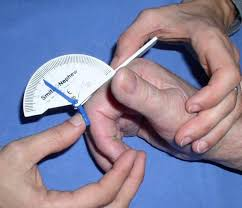
\includegraphics[width=0.4\textwidth]{./img/rehabAnti}
	\caption{Mecanismo de medición de los ángulos de apertura de las articulaciones de la mano. } 
	\label{fig:medidaAnticuada}
\end{figure} 


%--TECNOLOGIAS MEDICIÓN
\subsection{Tecnologías para la medición del movimiento}
\label{sec:tecnologias2}

En la actualidad existen diferentes sistemas que permiten medir el movimiento. Entre ellos podemos enumerar:
\begin{itemize}
	\item {Cámaras}
	\item {Fibras FBG}
	\item {IMU}
	\item {Sensores capacitivos}
	\item {Sensores mioeléctricos}
\end{itemize}

Teniendo en cuenta la aplicación de este trabajo, y las deformaciones que tienen las manos a medir las dos tecnologías que mejor se adaptan al problema son las fibras FBG y los sensores inerciales.

En este trabajo se estudian más en profundidad las fibras FBG y los sensores IMU. Para ello se han desarrollado un primer prototipo basado en las fibras de Bragg. Además, se ha propone un segundo prototipo basado en sensores inerciales. Notese que por prototipo se refiere a sistema hardware y software.

------------ ------------ ------------ ------------

\textcolor{rositaoscuro}{Por cierto, no hago referencia a explicar el proyecto de colaboraion entre adacen y la upna, debería?}

\textcolor{teal}{
Colaboración entre la Universidad Pública de Navarra (UPNA) y la Asociación del Daño Cerebral de Navarra	(ADACEN). 
}

\textcolor{teal}{
Fruto de esta propuesta de colaboración, se obtuvo financiación para la realización de un proyecto del Departamento de Desarrollo Económico del Gobierno de Navarra, cuya referencia es SENSMOV: “Sistema TIC de evaluación de la movilidad para personas con problemas motores”. Dicho proyecto comprende diferentes líneas de trabajo divididas en la obtención de prototipos. El primero de ellos, integra un conjunto de unidades inerciales para medir y evaluar el movimiento de las extremidades tanto superiores como inferiores. Un segundo prototipo considera un sensor de ultrasonidos de bajo coste para medir, por ejemplo, la distancia entre pasos o rangos de movimiento. Este último complementaría la información y datos obtenidos por el prototipo anterior. Finalmente, un tercer prototipo y objeto de este trabajo, trata de diseñar un guante de sensores de fibra óptica basado en redes de difracción Bragg (FBG) para monitorizar los movimientos de la mano y dedos con el objetivo de utilizarse como técnica para la rehabilitación del rango articular de la mano.
}

\textcolor{teal}{
En conjunto, los tres prototipos citados anteriormente, forman parte de un proyecto más amplio para apoyo al diagnóstico, usable en la mejora de la calidad, eficacia y eficiencia de la atención de pacientes de movilidad reducida. A su vez, reduciendo los costes asistenciales. Además, comprende la integración de los sistemas anteriores en un software capaz de analizar los datos obtenidos tras la monitorización del paciente. Siendo necesario generar protocolos de implementación profesional de todos los prototipos desarrollados a fin de garantizar una correcta aplicación.
}

 